\documentclass{beamer}

\usetheme{metropolis}
\usecolortheme{beaver} 
\usepackage{graphicx}
\graphicspath{ {./attachments} }

\usepackage{tikz}
\usepackage{minted}
\usepackage{amsmath}
\usepackage{amssymb}
\usepackage{environ}
\usepackage{xcolor}
\usepackage{animate}
\usepackage{subcaption}
\usetikzlibrary{shapes, shapes.geometric, arrows, arrows.meta, positioning, shadows, fit, calc}

\definecolor{softblue}{RGB}{79, 117, 139}   % Muted Slate Blue
\definecolor{softred}{RGB}{186, 92, 92}     % Muted Coral/Rose
\definecolor{softgreen}{RGB}{92, 138, 92}   % Sage Green
\definecolor{arrowgray}{RGB}{100, 100, 100} % Dark Grey for arrows

% \newenvironment{banner}{%
%   \begin{columns}[T]
%     \begin{column}{2.5cm}
%       \begin{tikzpicture}[remember picture,overlay]
%         \node[anchor=north west, inner sep=0pt] at (current page.north west) {%
%           \includegraphics[height=\paperheight]{banner.png}
%         };
%       \end{tikzpicture}
%     \end{column}
%     \begin{column}{0.85\textwidth}
% }{%
%     \end{column}
%   \end{columns}
% }

\title{Robot Automation}
\subtitle{Line Following Robot \\ Day 6}
\date{\today}

\begin{document}

\begin{frame}
    \titlepage
\end{frame}

% {
%     \usebackgroundtemplate{%
%         \includegraphics[width=\paperwidth,height=\paperheight]{background.jpg}%
%     }
%     \begin{frame}[plain]
%         \vspace{1em}

%         \begin{columns}[c] 
%             \begin{column}{0.54\textwidth}
%                 \hspace*{0.5cm}%
%                 \includegraphics[width=0.4\linewidth]{club_logo.png}
%             \end{column}
%             \begin{column}{0.52\textwidth}
%                 \hspace*{-0.5cm}%
%                 \includegraphics[width=0.9\linewidth]{locus.png}
%             \end{column}
%         \end{columns}

%         \vfill

%         \centering
%         \color{white} 
%         {\Huge \textbf{Hardware Fellowship}}\\
% 		{\Huge \textbf{Day 6}}\\
% 		\vspace{1em}
% 		{\Large \textbf{Robot Automation}}\\
        
%         \vspace{1em} 
%     \end{frame}
% } 

\begin{frame}
	\tableofcontents
\end{frame}

\section{Introduction to Robot Automation}

\begin{frame}{What is Robot Automation?}
% \begin{banner}
	Robot Automation can simply be defined as any means by which a robotic system performs a given task without any external intervention.
	\vfill
	\begin{figure}[h]
		\centering
        \animategraphics[loop, autoplay,  height=0.55\textheight]{8}{./attachments/roomba/roomba-}{0}{21}
		\caption{A roomba cleaning the floor}
	\end{figure}
% \end{banner}
\end{frame}

\begin{frame}{What is Robot Automation?}
% \begin{banner}
	This is usually achieved by informing the robot of its current state using various sensors. Then, aware of its state, the robot uses various algorithms such that the robot decides on its own the next optimal steps it should take to achieve its desired goal. These algorithms are known as \textbf{Control Systems}.
% \end{banner}
\end{frame}

\begin{frame}{Parts of an Automatic Robot}
	\begin{itemize}
		\item \textbf{Sensors}
		\item \textbf{Control Systems}(Algorithms)
		\item \textbf{Mechanical Actuation}
	\end{itemize}
	Today, we are only concerned with the data acquision by the \textit{sensors} as well as the \textit{control} systems that will be used to control the robot.
\end{frame}


\begin{frame}{Robot Component Interaction}
    \centering
    \resizebox{0.85\textwidth}{!}{%
	    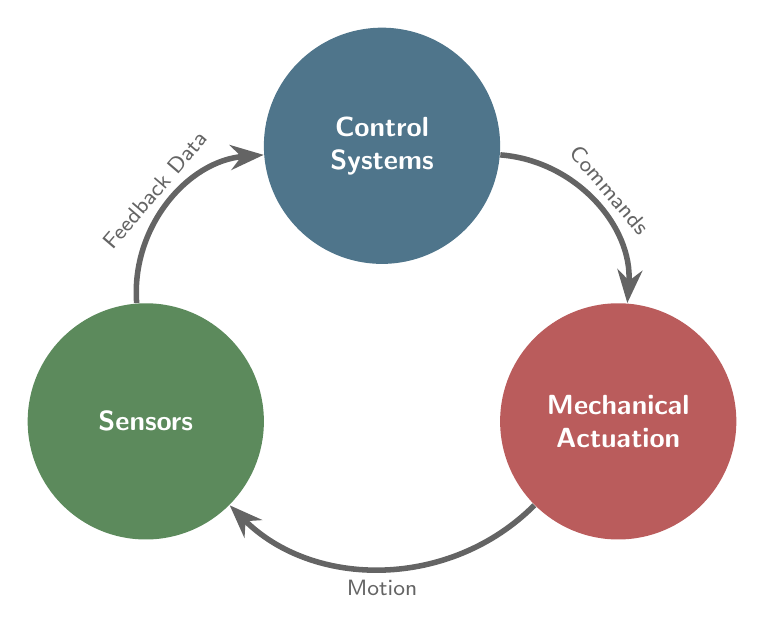
\begin{tikzpicture}[
	        node distance=2.5cm,
	        font=\sffamily\bfseries,
	        component/.style={
	            circle,
	            minimum size=3cm,
	            text width=2.5cm,
	            align=center,
	            draw=none,
	            text=white,
	        },
	        flow/.style={
	            -Stealth, 
	            line width=2pt, 
	            draw=arrowgray,
	            bend left=45
	        },
	        labeltext/.style={
	            text=arrowgray,
	            font=\sffamily\footnotesize,
	            align=center
	        }
	    ]
	        \node[component, fill=softblue] (control) at (0, 0) {Control\\Systems};
	        \node[component, fill=softred] (actuation) at (3, -3.5) {Mechanical\\Actuation};
	        \node[component, fill=softgreen] (sensors) at (-3, -3.5) {Sensors};

	        \draw[flow] (control) to node[labeltext, midway, sloped, above] {Commands} (actuation);
	        \draw[flow] (actuation) to node[labeltext, midway, sloped, below] {Motion} (sensors);
	        \draw[flow] (sensors) to node[labeltext, midway, sloped, above] {Feedback Data} (control);
	    \end{tikzpicture}
    }
\end{frame}

\section{The IR Sensor}

\begin{frame}{Working Principle}
	\begin{figure}[h]
		\includegraphics[scale=0.18]{ir_sensor.jpg}
	\end{figure}
	An IR sensor uses an \textbf{IR LED} and a \textbf{Photodiode} to detect objects.
	\begin{itemize}
		\item The \textbf{IR LED} emits infrared light.
		\item When an object comes close, this light reflects back.
		\item The \textbf{Photodiode} receives the reflected light.
		\item The module processes this change and gives corresponding output on its \textbf{OUT} pin.
	\end{itemize}
\end{frame}

\begin{frame}{Line Detection}
	The key insight to using this sensor for detecting a line is that the amount of light that gets reflected back depends on the reflectivity of the surface. The reflectivity in turn is dependent on the color of the surface.
	\begin{itemize}
		\item Light surfaces reflect more light back.
		\item Dark surfaces reflect less light back.
	\end{itemize}
\end{frame}

\begin{frame}{Interfacing with the IR sensor}
	\begin{itemize}
		\item Connect \textbf{VCC} of the IR sensor to 5V of the ESP32.
		\item Connect \textbf{GND} of the IR sensor to GND of the ESP32.
		\item Connect \textbf{OUT} pin of the IR sensor to any digital input pin on the ESP32.
	\end{itemize}
\end{frame}

\begin{frame}{Interfacing with the IR sensor}
	\begin{itemize}
		\item The IR sensor we have has an \textbf{Active Low} output. Therefore we will get a \textbf{LOW} output when an object is detected and a \textbf{HIGH} output when an object is not detected.
		\item The distance at which the object gets detected can be changed by adjusting the \textbf{potentiometer} on the IR sensor.
		\item Additionally, an indicator led is also present in the sensor which will light up when an object gets detected.
	\end{itemize}
\end{frame}

\begin{frame}[fragile]{Code Snippet}
	\begin{minted}{C++}
int irPin = 2;  // Digital pin connected to IR sensor

void setup() {
  pinMode(irPin, INPUT_PULLUP);
  Serial.begin(9600);
}

void loop() {
  int state = digitalRead(irPin);
  Serial.println(state);
  delay(200);
}
	\end{minted}
\end{frame}

\section{Robot Overview}
\begin{frame}{System Architecture}
    \centering
    \resizebox{\textwidth}{!}{
    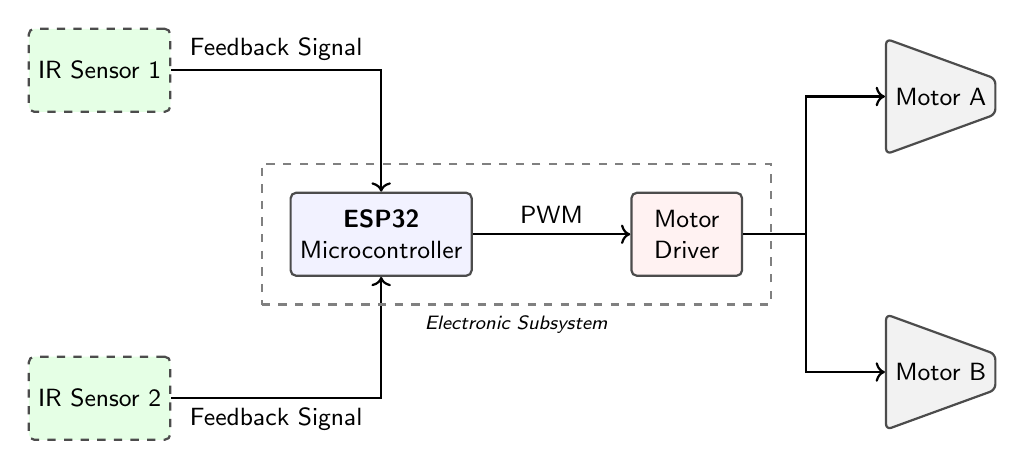
\begin{tikzpicture}[
        auto,
        node distance = 1.5cm and 2cm,
        thick,
        font=\sffamily\small,
        block/.style = {
            draw=black!70, 
            fill=blue!5, 
            rectangle, 
            rounded corners=2pt, 
            minimum height=3em, 
            minimum width=4em, 
            align=center,
        },
        sensor_node/.style = {
            block,
            fill=green!10,
            dashed 
        },
        motor_node/.style = {
            block,
            fill=gray!10,
            shape=trapezium, 
            shape border rotate=270,
            trapezium angle=70
        }
    ]

	    \node[block] (esp) {\textbf{ESP32}\\Microcontroller};

	    \node[sensor_node, above left=1cm and 1.5cm of esp] (ir1) {IR Sensor 1};
	    \node[sensor_node, below left=1cm and 1.5cm of esp] (ir2) {IR Sensor 2};

	    \node[block, right=of esp, fill=red!5] (driver) {Motor\\Driver};

	    \node[motor_node, above right=0.5cm and 1.8cm of driver] (m1) {Motor A};
	    \node[motor_node, below right=0.5cm and 1.8cm of driver] (m2) {Motor B};

	    \draw[->] (ir1) -| node[near start, above] {Feedback Signal} (esp);
	    \draw[->] (ir2) -| node[near start, below] {Feedback Signal} (esp);

	    \draw[->] (esp) -- node[above] {PWM} (driver);

	    \draw[->] (driver.east) -- ++(0.8,0) |- (m1.west);
	    \draw[->] (driver.east) -- ++(0.8,0) |- (m2.west);

	    \node[draw=gray, dashed, inner sep=10pt, fit=(esp) (driver), label=below:\textit{\scriptsize Electronic Subsystem}] {};

    \end{tikzpicture}
	}
\end{frame}

\begin{frame}{Data Acquisition}
	\begin{itemize}
		\item We should acquire and store the \textit{feedback signals} from both IR sensors into their own variables.
		\item Then by knowing which sensor's data (\textit{left or right}) a variable refers to, we can know which side of the line we are on.
	\end{itemize}
\end{frame}

\begin{frame}[fragile]{Code Snippet}
	\begin{minted}[
		fontsize=\scriptsize,
		breaklines=true,
	]{C++}
int ir1 = 2;  // Digital pin connected to the left IR sensor
int ir2 = 6;  // Digital pin connected to the right IR sensor

void setup() {
  pinMode(ir1, INPUT_PULLUP);
  pinMode(ir2, INPUT_PULLUP);
  Serial.begin(9600);
}

void loop() {
  int ir1_state = digitaRead(ir1);
  int ir2_state = digitaRead(ir2);
  if (ir1_state == 0 && ir2_state == 1) {
	Serial.println("Line on Right Side");
  }
  if (ir1_state == 1 && ir2_state == 0) {
	Serial.println("Line on Left Side");
  }
  delay(100);
}
	\end{minted}
\end{frame}

\section{Introduction to Control Systems}

\begin{frame}{Brief Introduction to Control Systems}
	\begin{itemize}
		\item Control Systems are a set of algorithms and mechanisms used to \textit{control} the behaviour of a given physical process.
		\item Most Control Systems use \textbf{feedback}. That is, they measure the actual output of the system using sensors and compare the actual output to the desired output called the \textit{setpoint}.
		\item They use the difference between the desired output and the \textit{setpoint} called the \textit{error} to choose the optimal next step to take.
	\end{itemize}
\end{frame}

\begin{frame}{Feedback Loop}
  \centering
    
    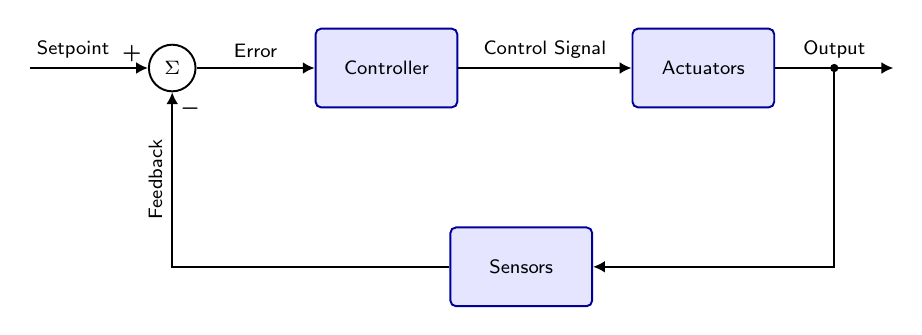
\begin{tikzpicture}[
        auto, 
        node distance = 1cm and 1.5cm,
        > = {Latex[width=1.5mm,length=1.5mm]},
        line width = 0.7pt,
        block/.style = {
            draw, 
            rectangle, 
            minimum height = 1cm, 
            minimum width = 1.8cm, 
            align = center, 
            fill = blue!10,
            draw = blue!60!black,
            rounded corners = 2pt,
            font = \sffamily\scriptsize
        },
        sum/.style = {
            draw, 
            circle, 
            minimum size = 0.5cm, 
            fill = white, 
            draw = black
        },
        point/.style = {coordinate},
        every node/.style={font=\sffamily\scriptsize}
    ]

        \node[point] (input) {};
        \node[sum, right=of input] (sum) {$\Sigma$};
        \node[block, right=of sum] (controller) {Controller};
        \node[block, right=2.2cm of controller] (plant) {Actuators};

		\coordinate (Mid) at ($($(controller.south)!0.5!(plant.south)$) + (-0.3cm, -1.5cm)$);

		\node[block, anchor=north] (sensor) at (Mid) {Sensors};
        \node[point, right=of plant] (output) {};

        \draw[->] (input) -- node[above, xshift=-0.2cm] {Setpoint} (sum);
        
        \draw[->] (sum) -- node[above] {Error} (controller);
        \draw[->] (controller) -- node[above] {Control Signal} (plant);
        
        \draw[->] (plant) -- node[above] {Output} coordinate[midway] (branch) (output);

        \fill (branch) circle (1.5pt);
        \draw[->] (branch) |- (sensor);
        
        \draw[->] (sensor) -| 
            node[pos=0.75, rotate=90, above] {Feedback} 
            (sum);

        \node[above left=-2pt] at (sum.west) {$\boldsymbol{+}$};
        \node[below right=-1pt] at (sum.south) {$\boldsymbol{-}$};

    \end{tikzpicture}
\end{frame}

\begin{frame}{Example of Control System}
	An example of a Control System is the \textbf{Thrust Vectoring} used in rockets and figher jets.
	\begin{figure}[h]
		\centering
        \animategraphics[loop, autoplay, height=0.6\textheight]{12}{./attachments/thrust_vectoring/frame-}{0}{39}
		\caption{A multi-axis thrust vectoring engine nozzle in motion}
	\end{figure}
\end{frame}

\begin{frame}{Thrust Vectoring}
	\begin{figure}[h]
	    \centering
	    \begin{subfigure}[b]{0.45\textwidth}
	        \centering
	        \includegraphics[width=\textwidth]{thrust_vector_diagram.png}
	        \caption{Moments generated by different thrust angles}
	    \end{subfigure}
	    \hfill
	    \begin{subfigure}[b]{0.45\textwidth}
	        \centering
	        \includegraphics[width=\textwidth]{f35.jpg}
	        \caption{F35-B Fighter Jet taking off with thrust-vectored nozzle}
	    \end{subfigure}
	\end{figure}
\end{frame}

\section{Algorithm Design}

\begin{frame}{System Realization}
	\begin{itemize}
		\item Our objective is for the robot to travel along the line while keeping the line as close to its center as possible.
		\item The simplest approach is to move the robot in the direction of the line. That is, move the robot to the left if the line is to the left and move the robot to the right if the line is to the right.
		\item This is the simplest feedback Control System known as \textbf{On-Off Control} or \textbf{Bang-Bang Control}.
	\end{itemize}
\end{frame}

\begin{frame}{Line Follower Algorithm}
    \centering
    \resizebox{!}{0.9\textheight}{%
        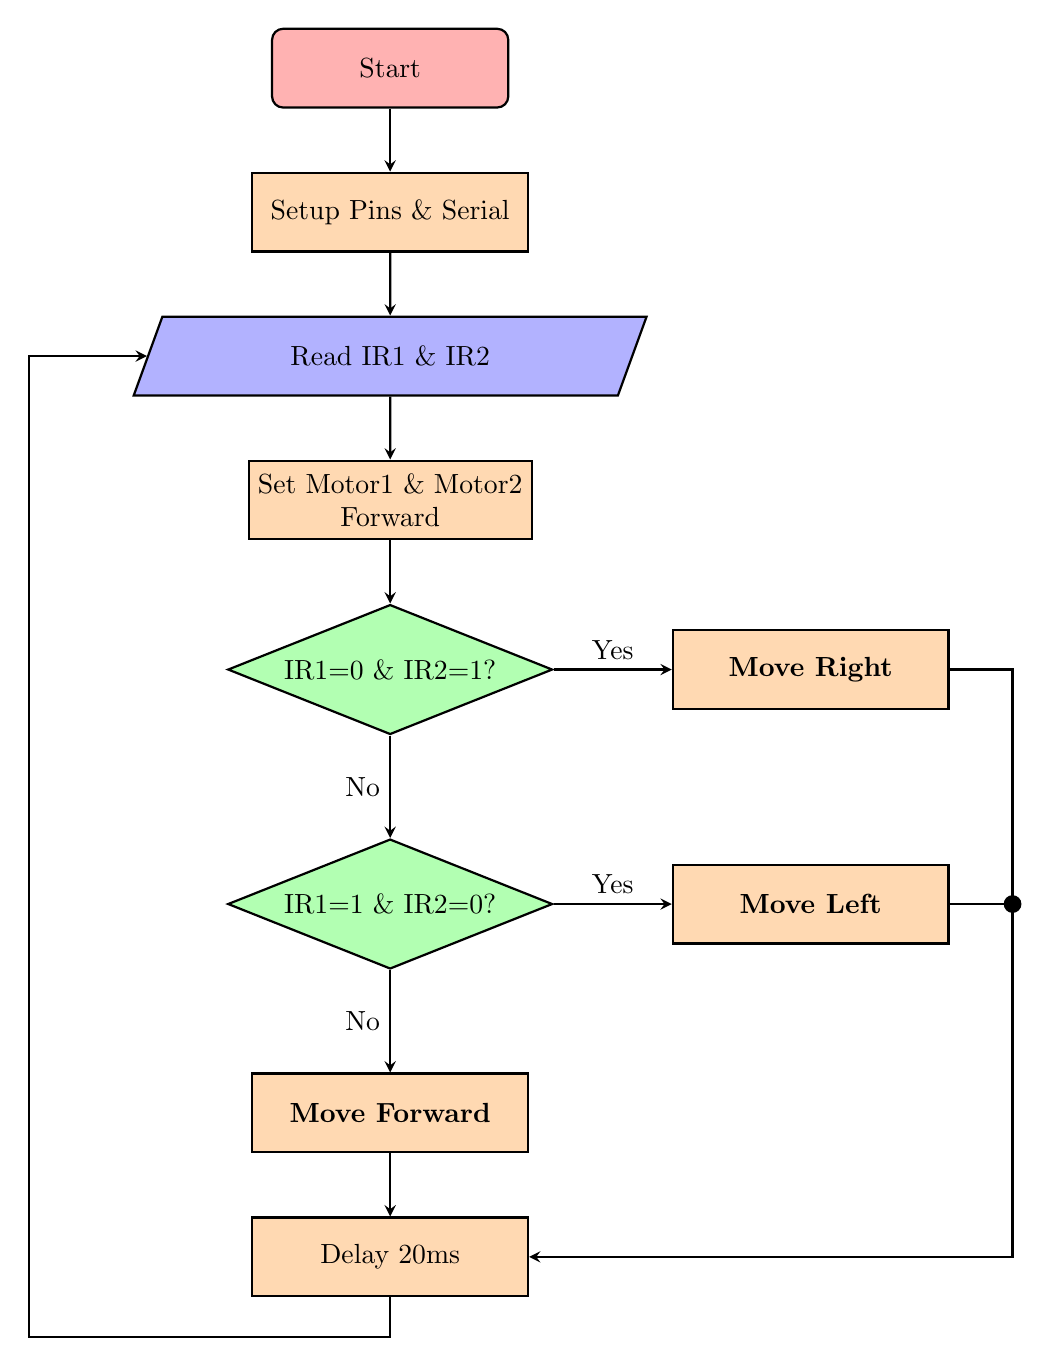
\begin{tikzpicture}[
            node distance=0.8cm and 1.5cm,
            auto,
			>={stealth},
            startstop/.style={
				rectangle,
				rounded corners,
				minimum width=3cm,
				minimum height=1cm,
				align=center,
				draw=black,
				thick,
				fill=red!30
			},
            io/.style={
				trapezium,
				trapezium left angle=70,
				trapezium right angle=110,
				minimum width=3cm,
				minimum height=1cm,
				align=center,
				draw=black,
				thick,
				fill=blue!30
			},
            process/.style={
				rectangle,
				minimum width=3.5cm,
				minimum height=1cm,
				align=center,
				draw=black,
				thick,
				fill=orange!30
			},
            decision/.style={
				diamond,
				aspect=2.5,
				minimum width=3cm,
				minimum height=0.8cm,
				align=center,
				draw=black,
				thick,
				fill=green!30
			},
            arrow/.style={
				thick,
				->
			},
            line/.style={
				thick
			} 
        ]

        \node (start) [startstop] {Start};
        \node (setup) [process, below=of start] {Setup Pins \& Serial};
        \node (read) [io, below=of setup] {Read IR1 \& IR2};
        \node (motorsOn) [process, below=of read] {Set Motor1 \& Motor2\\Forward};
        \node (dec1) [decision, below=of motorsOn] {IR1=0 \& IR2=1?};
        \node (dec2) [decision, below=of dec1, yshift=-0.5cm] {IR1=1 \& IR2=0?};
        \node (fwd) [process, below=of dec2, yshift=-0.5cm] {\textbf{Move Forward}};
        \node (delay) [process, below=of fwd] {Delay 20ms};

        \node (right) [process, right=of dec1] {\textbf{Move Right}};
        \node (left) [process, right=of dec2] {\textbf{Move Left}};

        \draw [arrow] (start) -- (setup);
        \draw [arrow] (setup) -- (read);
        \draw [arrow] (read) -- (motorsOn);
        \draw [arrow] (motorsOn) -- (dec1);
        \draw [arrow] (dec1) -- node[left] {No} (dec2);
        \draw [arrow] (dec2) -- node[left] {No} (fwd);
        \draw [arrow] (fwd) -- (delay);
        \draw [arrow] (dec1) -- node[above] {Yes} (right);
        \draw [arrow] (dec2) -- node[above] {Yes} (left);

        \coordinate (commonLine) at ($(right.east) + (0.8, 0)$);
        
        \coordinate (intersection) at (commonLine |- left.east);

        \draw [line] (right.east) -| (intersection);

        \draw [line] (left.east) -- (intersection);

        \filldraw[black] (intersection) circle (3pt);

        \draw [arrow] (intersection) |- (delay.east);

        \draw [arrow] (delay.south) -- ++(0,-0.5) -| ([xshift=-1.5cm]read.west) -- (read.west);

        \end{tikzpicture}
    }
\end{frame}

\begin{frame}[fragile]{Code: Connection Initialization}
	\begin{minted}[
		fontsize=\scriptsize,
		breaklines=true,
	]{C++}
// IR sensors connection
int ir1 = 2; 
int ir2 = 6;  

// Motor A connections
int enA = 9;
int in1 = 8;
int in2 = 7;

// Motor B connections
int enB = 3;
int in3 = 5;
int in4 = 4;

// PWMs for motors
int full_speed = 200;
int slow_speed = 100;
	\end{minted}
\end{frame}

\begin{frame}[fragile]{Code: Initialization}
	\begin{minted}[
		fontsize=\scriptsize,
		breaklines=true,
	]{C++}
void setup() {
  pinMode(ir1, INPUT_PULLUP);
  pinMode(ir2, INPUT_PULLUP);

  // Set all the motor control pins to outputs
  pinMode(enA, OUTPUT);
  pinMode(enB, OUTPUT);
  pinMode(in1, OUTPUT);
  pinMode(in2, OUTPUT);
  pinMode(in3, OUTPUT);
  pinMode(in4, OUTPUT);

  // Turn off motors - Initial state
  digitalWrite(in1, LOW);
  digitalWrite(in2, LOW);
  digitalWrite(in3, LOW);
  digitalWrite(in4, LOW);
  Serial.begin(9600);
}
	\end{minted}
\end{frame}

\begin{frame}[fragile]{Code: Helper Functions}
	\begin{minted}[
		fontsize=\scriptsize,
		breaklines=true,
	]{C++}
void move_left() {
  analogWrite(m1_pwm, slow_speed);
  analogWrite(m2_pwm, full_speed);
}

void move_right() {
  analogWrite(m1_pwm, full_speed);
  analogWrite(m2_pwm, slow_speed);
}

void move_forward() {
  analogWrite(m1_pwm, full_speed);
  analogWrite(m2_pwm, full_speed);
}
	\end{minted}
\end{frame}

\begin{frame}[fragile]{Code: Main Body}
	\begin{minted}[
		fontsize=\scriptsize,
		breaklines=true,
	]{C++}
void loop() {
  int ir1_state = digitaRead(ir1);
  int ir2_state = digitaRead(ir2);

  // Turn on Motors
  digitalWrite(in1, HIGH);
  digitalWrite(in2, LOW);
  digitalWrite(in3, HIGH);
  digitalWrite(in4, LOW);

  if (ir1_state == 0 && ir2_state == 1) {
	move_right();
  }
  else if (ir1_state == 1 && ir2_state == 0) {
	move_left();
  }
  else {
	move_forward();
  }
  delay(20);
}
	\end{minted}
\end{frame}

\end{document}
